\documentclass{article}
\usepackage{indentfirst}
\usepackage{lmodern}
\usepackage[utf8]{inputenc}
\usepackage[T1]{fontenc}
\usepackage[ngerman]{babel}
\usepackage{amssymb,amstext,amsmath}
\usepackage{graphicx}
\usepackage{dsfont}
\usepackage{amsfonts}
\usepackage{graphics}
\usepackage{float}
\usepackage{cite}
\usepackage{url}
\usepackage{tabularx}
\usepackage{capt-of}

\title{Photoemission}
\author{Alexander Heinisch, Dominik Wille}
\begin{document}
\maketitle
\vspace{13cm}
\noindent
\begin{center}
\begin{tabular}{r l}
Tutor & Heimberger\\
Durchführung & 29. Mai 2013 von 14-18 Uhr \\

E-Mail Dominik & dominik.wille@fu-berlin.de \\
E-Mail Alexander & matthias.heinisch@gmx.de \\
\end{tabular}
\end{center}

\newpage
\tableofcontents
\newpage

\section{Physikalische Grundlagen}

\subsection{Hallwachs-Effekt}
Ende des 19. Jahrhunderts entdeckte Wilhelm Hallwachs, dass die Bestrahlung einer Metallplatte mit kurzwelligem Licht eine Ladungstrennung zur Folge hat. Die Platte lädt sich dabei durch die Abgabe von negativen Ladungen, bis zu einer gewissen Spannung, positiv auf. Ist dieses Haltepotential erreicht, werden weitere ausgelöste Ladungen zurückgehalten (Hallwachs-Effekt). Später fand man heraus, dass die herausgelösten Ladungen Elektronen sind (Photoemission).
Diese Entdeckung stand im Widerspruch zur damals gängigen Wellentheorie des Lichts und durch intensive Untersuchungen gelangte man zu folgenden Ergebnissen:

\begin{itemize}
\item Der Effekt tritt instatan auf
\item Es gibt einen proportionalen Zusammenhang zwischen dem Sättigungsstrom und der Intensität des Lichts
\item Es gibt keinen Zusammenhang zwischen der Intensität des Lichts und der kinetischen Energie der herausgelösten Elektronen
\item Je höher die Frequenz des Lichts, desto höher ist die kinetische Energie der Elektronen
\item Die Frequenz muss einen Minimalwert überschreiten, damit der Effekt eintritt (langweilige Frequenz)
\end{itemize}

\subsection{Licht-Quantentheorie}
Aufgrund der Unstimmigkeiten der Wellentheorie des Lichts mit den neuen Entdeckungen, schlug Albert Einstein 1905 eine neue Korpuskulartheorie des Lichts vor.\\
Licht besteht aus Lichtquanten, welche sich geradlinig mit der Geschwindigkeit c bewegen. In Abhängigkeit der Frequenz, tragen die Quanten dabei eine Energie von \(h\cdot \nu\). Kommt es nun zur Photoemission, wird die gesamte Energie des Lichtteilchens in Form von kinetischer Energie und verrichteter Austrittsarbeit auf das Elektron übertragen. 

\subsection{Austrittsarbeit}
Um ein Elektron aus einem (metallenem) Festkörper zu lösen, muss ihm Energie zugeführt werden. Die dabei benötigte Menge an Energie nennt man Austrittsarbeit. Je nach Metall, benötigt man weniger Energie (etwa 2eV im Frequenzbereich des sichtbaren Lichts für Alkalimetalle) oder mehr Energie (4-5eV im ultravioletten Bereich), um die langweilige Grenze zu erreichen. 

\subsection{Experimentelle Anordnung}
Der einfachste experimentelle Aufbau einer Photozelle, besteht aus einer flächenförmigen Kathode und einer Gegenelektrode. Die Kathode wir aus dem zu untersuchenden Material bestehen und die Elektrode das Gegenpotential aufbauen und den Photostrom auffangen.

\begin{center}
\begin{minipage}{\linewidth}
\centering
\makebox[0cm]{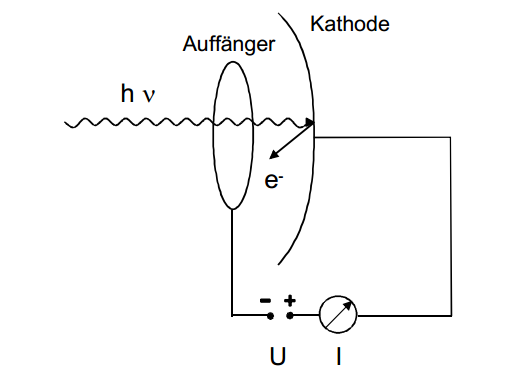
\includegraphics[width=8cm]{bilder/pho1}}
\captionof{figure}{Prinzipschaltskizze einer Photozelle [GP2-Skript]}%
\label{photozelle}
\end{minipage}
\end{center}

In der Skizze werden Elektronen durch den von links kommenden Photonenstrom der Energie \(h\cdot \nu\) aus der Kathode gelöst. Um die freien Elektronen aufzufangen, wird an der Elektrode eine Spannung U angelegt, durch welche auch der Photonenstrom \(I_{Ph}\) gemessen werden kann. Meistens werden Alkalimetalle für diese Experimente benutzt, da der Quantenausbeute bei ihnen ziemlich hoch ist (Verhältnis zwischen Photonen und emittierten Elektronen). Die beobachtbare Ströme werden im Bereich von \(10^{-12}\) bis \(10^{-9}\) Ampere liegen.
\newpage
\section{Aufgaben}

\subsection{Aufgabe 1}
Aufbau und Justierung der Apparatur

\subsection{Aufgabe 2}
Messung des Sättigungsstromes und der Bremsspannung einer Kalium-Photozelle in Abhängigkeit von der Beleuchtungsstärke für die 436-nm-Linie Iindigo/blau) von Quecksilber.

\subsection{Aufgabe 3}
Aufnahme der Strom-Spannungs-Kennlinien für alle Hauptlinien des Quecksilber-Spektrums. Auswertung der Kennlinien und Bestimmung des Plankschen Wirkungsquantums und der Austrittsarbeit von Kalium.

\subsection{Aufgabe 4}
Theoretische Aufgabe für die Ausarbeitung: Darstellung der Widersprüche zwischen den experimentellen Ergebnissen der Photoemission und der klassischen Wellentheorie des Lichts.

\newpage
\section{Quellenangabe}
\begin{itemize}
\item GPII-Skript
\item Platzskript
\item Abbildung 1: \(http://www.gesundheit.de/sites/default/files/images/roche/pics/a22297.000-1_big.gif\)
\item Abbildung 2:  \(http://www.gesundheit.de/sites/default/files/images/roche/pics/a22297.000-1_big.gif\)
\end{itemize}

\newpage
\end{document}